\documentclass[a4paper,12pt]{article}

% Packages
\usepackage[utf8]{inputenc}
\usepackage{amsmath, amssymb}
\usepackage{graphicx}
\usepackage{float}
\usepackage{hyperref}
\usepackage{geometry}
\usepackage{indentfirst}
\usepackage[backend=biber]{biblatex}
\addbibresource{references.bib} % Name of your .bib file
\geometry{margin=1in}



% Title and Author
\title{Zeeman Effect}
\author{Henry Su, Wen Hong Lou\\ NTU Physics Department}
\date{\today}

\begin{document}

\maketitle

\begin{abstract}
This report investigates the Zeeman Effect, a phenomenon where spectral lines are split into multiple components in the presence of a magnetic field. The experiment aims to measure the splitting and verify the theoretical predictions. 
\end{abstract}

\tableofcontents
\newpage

\section{Introduction}
The Zeeman effect, discovered by Pieter Zeeman in 1896, is the splitting of atomic spectral lines in the presence of a magnetic field. This experiment investigates both the normal and anomalous Zeeman effects, demonstrating how magnetic fields influence atomic energy levels. Using a cadmium lamp and a Fabry-Perot interferometer, we will observe the shifts in wavelength caused by the interaction of electron magnetic moments with an external magnetic field. Additionally, we will calculate the Bohr magneton, a fundamental physical constant that quantifies the magnetic moment of an electron due to its orbital or spin motion. This study enhances our understanding of atomic structure and the fundamental principles of quantum mechanics.\section{Theory}
\subsection{Zeeman Effect}
Zeeman effect is a phenomenon that an atomic spectral line is split into several components in the presence of a magnetic field. The splitting occurs due to the interaction between the magnetic moment of the atom and the external magnetic field. The effect can be classified into two types: normal and anomalous Zeeman effects. We'll get into the details of these two types in the latter section. But for now let us focus on the basic theory of the Zeeman effect. In the presence of weak magnetic field $\mathrm{B}$ the perturbed Hamiltonian can be written as follows:
\begin{equation}
H' = -\bold{\mu} \cdot \bold{B} = -\mu_B \bold{J} \cdot \bold{B} , ~~~ \mu_B = \frac{e \hbar}{2 m_e} = 9.274 \times 10^{-24} \mathrm{J/T}
\end{equation}
where $\vec{\mu}$ is the magnetic moment, $\mu_B$ is the Bohr magneton, and $\bold{J}$ is the total angular momentum of the atom. In particular, $\bold{J} = \bold{L} + 2\bold{S}$ where the factor 2 is the g-factor for the electron spin. In the latter on experiments our goal is to calculate Bohr magneton through energy level spliting. \\
\indent  Now let's consider the energy of the perturbed Hamiltonian by firt order perturbation theory. The "good state" of the perturtion is the normalized eigenbasis of the unperturbed Hamiltonian($H_0$), and it's charaterized mainly by magnetic quantum number $m_j$ and orbital quantum number $\ell$. With $\bold{B} = \mathrm{B}\hat{z}$, the energy of the perturbed Hamiltonian can be written as: 
\begin{align}
    E_{mj} 
    &= \langle n \ell jm_j \mid H' \mid n\ell jm_j \rangle \\
    &= \mu_{B}\,B \biggl[
      1 + \frac{j\,(j+1) + s\,(s+1) - l\,(l+1)}{2\,j\,(j+1)}
    \biggr] \, m_{j} 
    = -\,g_j\,\mu_{B}\,B\,m_{j}.
\end{align}
where $g_j$ is the Landé g-factor.
\subsection{Selection Rules}
Dispite knowing physically all the possible energy level existed, naturally not all transitions between state is allowed. We know the selection rule coonstrains the possible transitions between these energy states. There are two types of transitions allowed: 
\begin{align}
    \text{$\pi$-line : }&\Delta m_j = \pm 1\\ 
    \text{$\sigma_{\pm}$-line : }&\Delta m_j = 0 
\end{align}
\indent In our experimentm, we detected lights propagating parellel and perpendicular to the magnetic field $\bold{\mathrm{B}}$. Furthermore, the corrsponding two types of transitions to the light propagatind directions can be summurized in Fig.\ref{fig:zeeman_effect_1}
\begin{figure}[H]
    \centering
    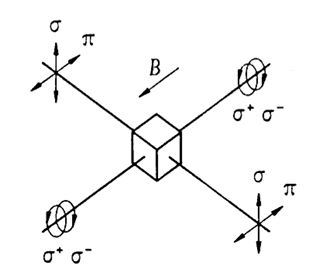
\includegraphics[width=0.5\textwidth]{Zeeman_effect_1.png}
    \caption{Illustration of the allowed transitions for the Zeeman effect, showing $\pi$-lines ($\Delta m_j = 0$) and $\sigma$-lines ($\Delta m_j = \pm 1$) for light propagating perpendicular to the magnetic field. Note that there is no $\pi$-line for light propagating parallel to the magnetic field because the magnetic dipole is oriented along the field. \cite{phyweZeeman}}
    \label{fig:zeeman_effect_1}
\end{figure}

\subsection{Normal and Anomalous Zeeman Effect}
\begin{equation}
    \mid i \rangle = \mid \ell_i, s_i, j_i, m_{j_i} \rangle \to \mid f \rangle = \mid \ell_f, s_f, j_f, m_{j_f} \rangle.
\end{equation}
\section{Experimental Setup and Procedure}
THIs is me.
Describe the f used, including the spectrometer, light source, and magnetic field generator. Include a diagram if possible:

\section{Procedure}
Outline the steps taken to perform the experiment, including calibration, data collection, and analysis.

\section{Results}
Present the observed spectral line splitting and compare it with theoretical predictions. Include tables and graphs where necessary.

\section{Discussion}
Analyze the results, discuss sources of error, and evaluate the agreement between experimental and theoretical values.

\section{Conclusion}
Summarize the findings and their implications for understanding the Zeeman Effect.

\section*{References}
\printbibliography

\end{document}